% !TeX root = ../thesis.tex

\chapter{Basisalgorithmus und Annahmen}
\label{sec:underlying-conditions_preliminaries}
Naumann und Stiller stellen in \cite{Naumann2017towards} einen Algorithmus zur kooperativen Verhaltensplanung automatisierter Fahrzeuge vor.
Dieser Algorithmus dient als Ausgangspunkt der vorliegenden Arbeit und soll im Weiteren als Basisalgorithmus bezeichnet werden.
In diesem Kapitel soll zun\"achst dieser Basisalgorithmus mit seinen wichtigsten Bestandteilen beschrieben werden.
Anschlie{\ss}end sollen Annahmen, die dem in dieser Arbeit vorgestellten Trajektorienplanungsalgorithmus zugrundeliegen, angegeben werden.


\section{Basisalgorithmus}
Naumann und Stiller \cite{Naumann2017towards} stellen einen Bewegungsplanungsalgorithmus vor, bei dem die Pr\"adiktion anderer Verkehrsteilnehmer in die Bewegungsplanung integriert wird.
Dies geschieht, indem im Optimierungsproblem nicht die Trajektorie Ego"=Fahrzeuges ermittelt wird, sondern die der anderen relevanten Fahrzeuge auch.
Das Ergebnis des Planungsalgorithmus ist demnach nicht mehr nur die optimale Trajektorie des Ego"=Fahrzeuges \gls{symb:x_optTra} \( = (x(t), y(t))^T \), sondern ein Trajektorienenset \gls{symb:x_Traset} \(= (\pmb{x}_1, \pmb{x}_2, ...) \), das aus den Trajektorien der einzelnen Fahrzeuge besteht.
Aus dem Optimierungsproblem wird somit ein Multi"=Agenten"=Optimierungsproblem.
Durch diese Multi"=Agenten"=Optimierung wird nicht nur ber\"ucksichtigt, dass andere Fahrzeuge das Verhalten des Ego"=Fahrzeuges beeinflussen sondern auch, dass das Ego"=Fahrzeug das Verhalten der anderen Verkehrsteilnehmer beeinflusst.
Die Verhaltensplanung des Ego"=Fahrzeuges ist damit nicht mehr rein reaktiv sondern kann nach \cite{Naumann2017} als kooperativ gewertet werden.

F\"ur dieses Mulit"=Agenten"=Optimierungsproblem wird ein neues Kostenfunktional vorgestellt, das au{\ss}er den Kosten des Ego"=Fahrzeuges auch die Kosten der anderen relevanten Fahrzeug enth\"alt.
Durch die Multi"=Agenten"=Optimierung ergibt sich ein stark nicht konvexes Optimierungsproblem, das nicht durch lokale Verfahren gel\"ost werden kann. 
Deshalb wird au{\ss}erdem ein globales, samplingbasiertes L\"osungsverfahren vorgestellt.
In den folgenden Abschnitten soll nun zun\"achst das Kostenfunktional des Basisalgorithmus vorgestellt werden. 
Anschlie{\ss}end sollen das samplingbasierte L\"osungsverfahren erl\"autert werden.

\subsection{Kostenfunktional}
\label{sec:Kostfunc}
Wie bereits erw\"ahnt soll in der Optimierung nicht nur das Ego"=Fahrzeug ber\"ucksichtig werden, sondern alle anderen relevanten Fahrzeuge auch.
Dadurch m\"ussen diese auch im Kostenfunktional ber\"ucksichtigt werden.
Gefunden werden sollen nun das Trajektorienset, dass die geringsten Gesamtkosten verursacht.
Daf\"ur wird ein Kostenfunktional eingef\"uhrt, dass sich aus der Summe der Kosten aller relevanten Verkehrsteilnehmer ergibt:

\begin{equation}
G_{total} = \sum_i G_i .
\end{equation}

Die Kosten \( G_i \) der einzelnen Fahrzeuge sollen zum einen gew\"ahrleisten, dass die Trajektorie durchf\"uhrbar und kollisionsfrei ist. 
Auf der anderen Seite sollen sie auch daf\"ur sorgen, dass komfortable Trajektorien generiert werden.
Die Kosten der einzelnen Fahrzeuge k\"onnen nochmal unterteilt werden:

\begin{equation}
G_i = G_{i,0} + \sum_j G_{i,j}.
\end{equation}

\( G_{i,0} \) sind Kosten die ausschlie{\ss}lich die eigene Trajektorie betreffen. 
Dazu geh\"oren beispielsweise Terme die das Abweichen von einer Wunschgeschwindigkeit oder Beschleunigungen bestrafen.
In \( G_{i,j} \) werden Kosten ber\"ucksichtigt, die in Interaktion mit anderen Fahrzeugen entstehen.
Dabei geht es in erster Linie darum Kollisionsfreiheit zu garantieren.
Hier Abst\"ande zu anderen Fahrzeugen betrachtet.
Aber auch Vorfahrtsregeln k\"onnen in diesen Kosten abgebildet werden.

Die  einzelnen Kostenterme werden in einer abschnittsweise definierten Funktion berechnet.
Daf\"ur werden die Kosten in drei Zonen eingeteilt:

\begin{itemize}
\item Komfortzone \gls{symb:Zone_komf}
\item Diskomfortzone \gls{symb:Zone_disc}
\item Unrealisierbarkeitszone \gls{symb:Zone_inf}
\end{itemize}

jeweils f\"ur eine positive und negative Abweichnung von einem festgelegten Optimum \gls{symb:f_opt}.
Ein erster Grenzwert \gls{symb:f_discstartp} gibt an, ab welchem Wert die Diskomfortzone bei einer positiven Abweichung von Optimum beginnt. 
Ein zweiter Grenzwert \gls{symb:f_infstartp} gibt den Beginn der Unrealisierbarkeitszone an.
Bei einer negativen Abweichung sind die Grenzwerte entsprechend \gls{symb:f_discstartn} und \gls{symb:f_infstartn}.
In jeder Zone kommen neue Kosten hinzu.
In der Komfortzone besteht die Funktion zur Berechnung des Kostenterms nur aus einer Funktionskomponente \gls{symb:G_comf}, welche die Kosten vergleichsweise geringf\"ugig ansteigen l\"asst.
Mit Beginn der Diskomfortzone kommt die Funktionskomponente \gls{symb:G_disc} hinzu. 
Sie sorgt f\"ur einen quadratischen Anstieg der Kosten.
Die Unrealisierbarkeitszone beinhaltet zus\"atzlich die Funktionskomponente \gls{symb:G_inf}.
Durch sie steigen die Kosten nahezu senkrecht an.

Es ergibt sich die abschnittsweise definiert Funktion
\begin{equation}
  G(f) = 
  \begin{cases} 
    G_\mathrm{comf}                         & \quad , f \in Z_\mathrm{comf}\\ 
    G_\mathrm{comf} + G_\mathrm{disc}              & \quad , f \in Z_\mathrm{disc}\\ 
    G_\mathrm{comf} + G_\mathrm{disc} + G_\mathrm{inf}    & \quad , f \in Z_\mathrm{inf}.
  \end{cases} 
  \label{eqn:Kostenfunktion}
\end{equation}

Die verschiedenen Funktionskomponenten sowie die Gesamtfunktion~\ref{eqn:Kostenfunktion} sind in Abbildung~\ref{fig:Kostenfuntion} dargestellt.

\begin{figure}[H]
    \centering
    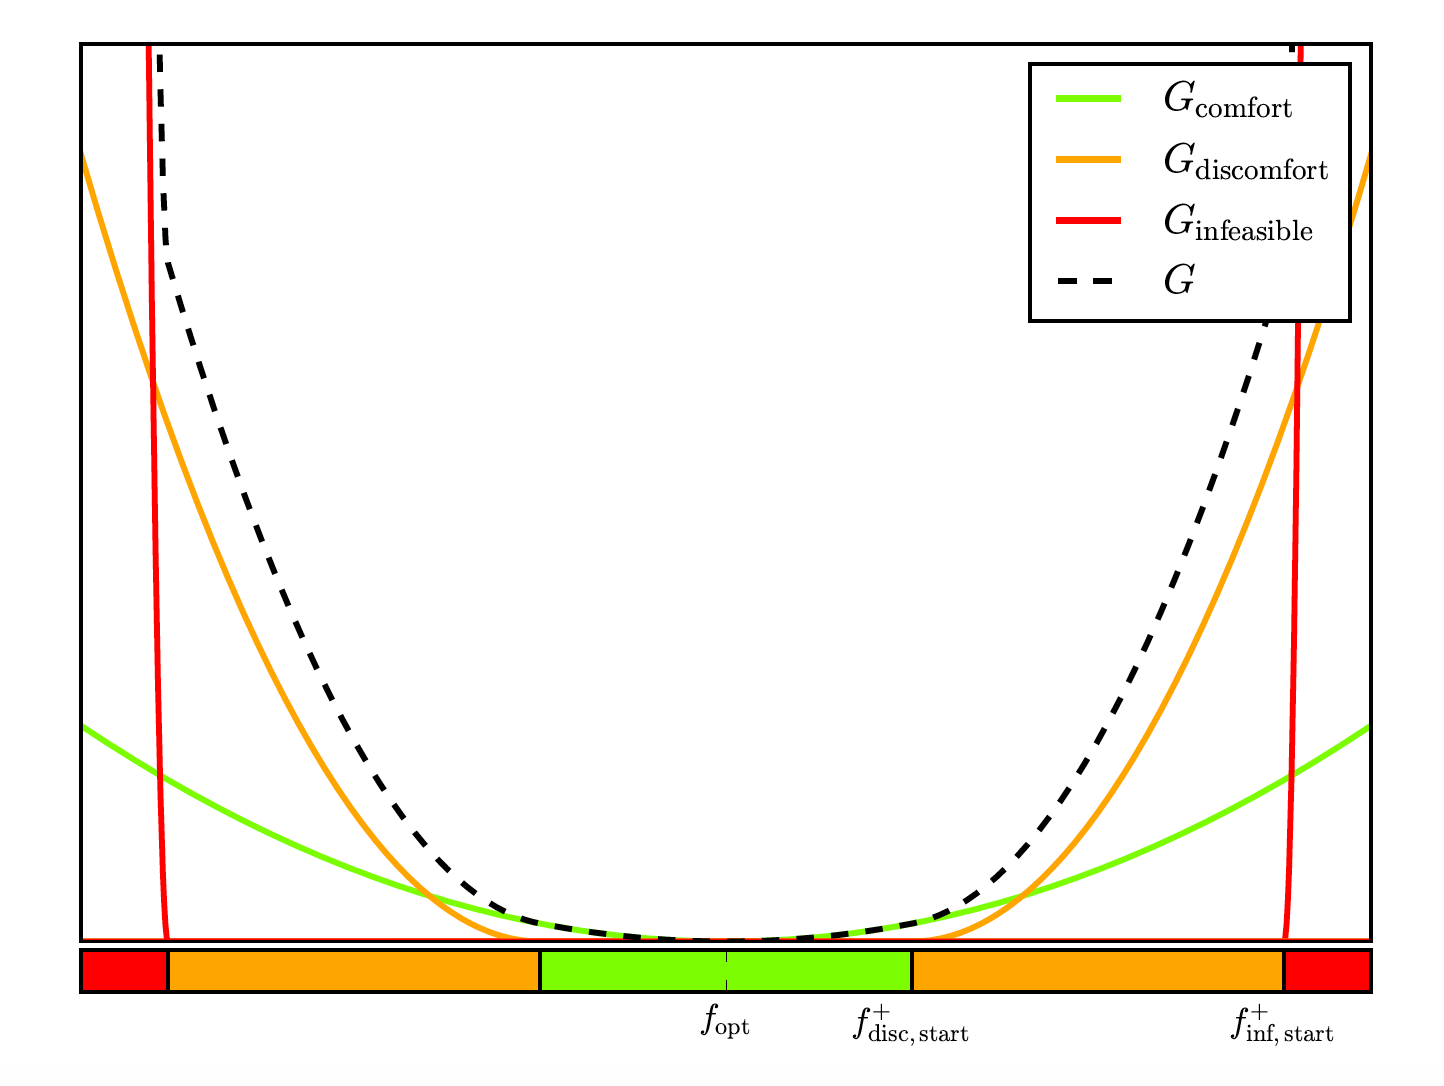
\includegraphics[width = 0.5 \textwidth ]{Kostenfuntion.png}
    \caption[Kostenfunktion]{Darstellung der Kostenfunktion}
    \label{fig:Kostenfuntion}
 \end{figure}


\subsection{Samplingbasiertes L\"osungsverfahren}
\label{sec:SmapPVD}
Wie bereits in Kapitel~\ref{globaleLV} erw\"ahnt bringt eine kooperative Trajektorienplanung meist ein nicht konvexes Optimierungsproblem mit sich.
Ein lokales L\"osungsverfahren k\"onnte nur bei einer starken Vereinfachung des Optimierungsproblems angewandet werden.
Es wird deshalb auf ein globales, samplingbasiertes L\"osungsverfahren zur\"uckgegriffen.
Da ein solches randomisiertes L\"osungsverfahren vergleichsweise uneffizient ist m\"ussen vereinfachende Annahmen getroffen werden, um das Ziel eines echtzeitf\"ahigen Algorithmus erreichbar zu machen.
Wie unter anderem in \cite{Ziegler2017}, \cite{Werling2011} und \cite{Rathgeber2016} kann sich auch hier zu Nutze gemacht werden, dass durch die Stra{\ss}e eine hochstrukturierte Umgebung gegeben ist.
Der Fahrkorridor ist dadurch weitestgehend eingeschr\"ankt.
In diesem Fall wird sich dies zu Nutze gemacht, indem auf die in \cite{Kant1986} vorgestellte \gls{pvd} zur\"urck gegriffen wird.
Hier findet die Trajektorienplanung in zwei separaten Schritten statt:

\begin{enumerate}
\item Generierung eines geometrischen Pfades der eine Kollision mit statischen Objekten vermeidet.
\item Generierung eines Geschwindigkeitsprofils f\"ur den gegebenen Pfad, sodass eine Kollision mit dynamischen Hindernissen vermieden wird.
\end{enumerate}

Der Pfad kann in vielen F\"allen als gegeben angenommen werden.
Eingeschr\"ankt durch die Fahrbahnmakierungen ergibt er sich oft durch die Fahrstreifenmitte. 
Soll nicht die Fahrstreifenmitte als Pfad angenommen werden kann auf bew\"ahrte Verfahren der Pfadgenerierung zur\"uck gegriffen werden.

Ist der Pfad bereits gegeben muss nun noch das Geschwindigkeitsprofil ermittelt werden.
Es ergibt sich somit eine eindimensionale Kontrollvariable.
Dadurch ist das Optimierungsproblem gut geeignet f\"ur ein Samplingverfahren.
Daf\"ur wird die gesuchten Trajektorien \gls{symb:x_optTra}(t) durch equidistante Zeitschritte diskretisiert:

\begin{equation}
\pmb{x}_k=\pmb{x}(t_k),   \quad t_k =t_0+k h
\end{equation}

mit der Diskretisierungsschrittweite \gls{symb:h}.
Um eine Trajektorie zu generieren wird nun f\"ur jeden Zeitschritt ein willk\"urlicher Ruck generiert.
Der Ruck ist die Ableitung der Beschleunigung.
Durch numerische Integration mittels des Finite"=Differenzen"=Verfahrens wird nun f\"ur jeden einzelnen Zeitschritt die Beschleunigung, Geschwindigkeit und die zur\"uckgelegte Wegstrecke entlang des Pfades berechnet werden.
Der Anfangszustand ist durch die Startbeschleunigung, -geschwindigkeit und -position gegeben.
Dieses Vorgehen ist in Abbildung~\ref{fig:Sampling} illustriert.
Zusammen mit dem im vorausgehenden Schritt generierten Pfad ergeben sich nun die Positionen \gls{symb:x_TraDisk} \( = (x_k, y_k)^T\) des Fahrzeuges an den einzelnen Zeitschritten und schlie{\ss}lich durch Interpolation zwischen den Zeitschritten die gesuchte Trajektorie \gls{symb:x_optTra}(t)\(= (x(t), y(t))^T\).

\begin{figure}[!htbp]
    \centering
    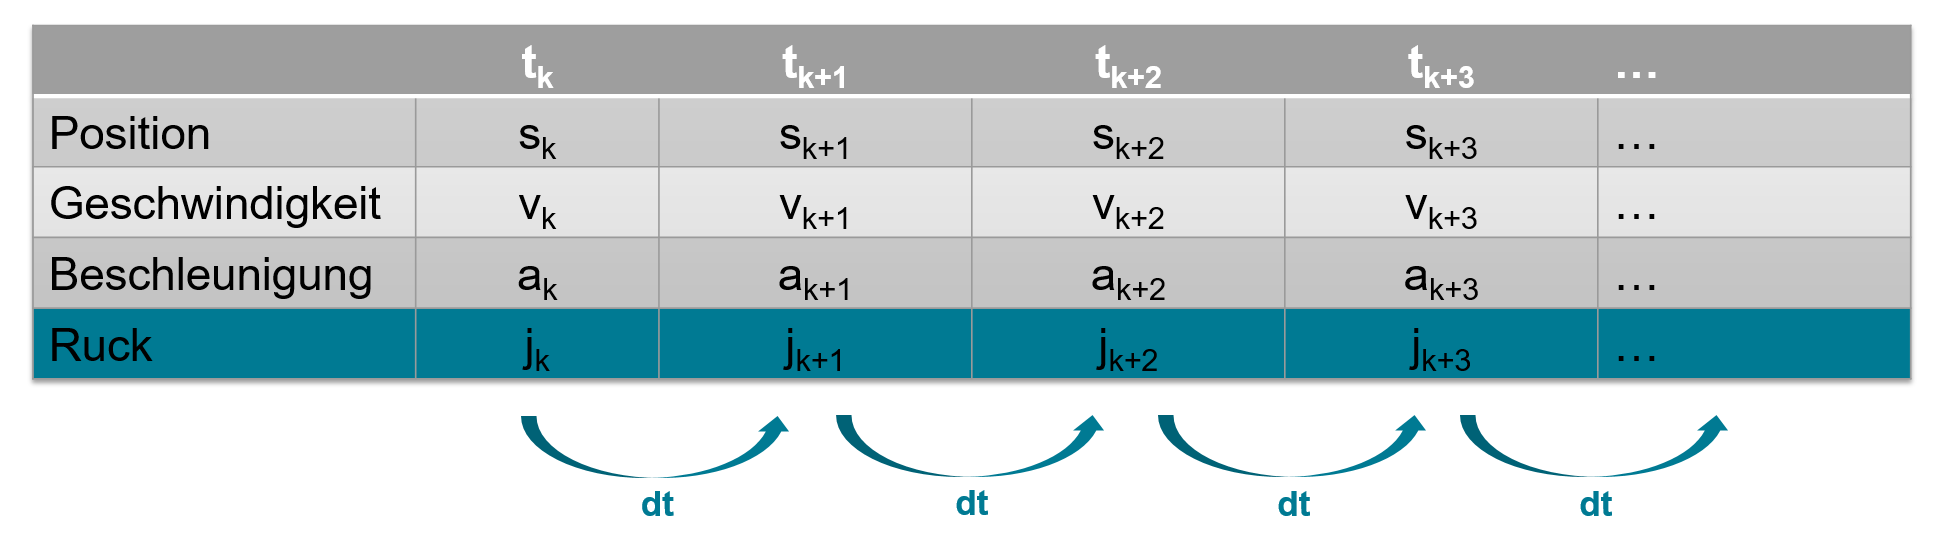
\includegraphics[width = 0.9 \textwidth ]{Sampling.png}
    \caption[Sampling]{Erzeugung eines Geschwindgkeitsprofils \"uber gesampelten Rucken}
    \label{fig:Sampling}
 \end{figure}

F\"ur jedes der beteiligten Fahrzeuge wird eine Vielzahl von Geschwindigkeitsprofilen und somit auch Trajektorien generiert.
Im Anschluss werden alle m\"oglichen Trajektorienkombinationen anhand des in Kapitel~\ref{sec:Kostfunc} vorgestellten Kostenfunktionals bewertet.
Die Trajektorienkombination mit den geringsten Kosten ergibt die angen\"aherte L\"osung des Multi"=Agenten"=Optimimierungsproblems.

Der Ruck wird zuf\"allig aus einem Wertebereich ermittelt, der durch einen vorgegeben maximalen und minimalen Ruck begrenzt ist.
Dadurch kann sicher gestellt werden, dass nur R\"ucke erzeugt werden die als komfortable empfunden werden.
Innere Nebenbedingungen wie maximal zul\"assige Geschwindigkeiten oder Beschleunigungen werden ber\"ucksichtigt, indem der zul\"assige Berreich des Rucks noch weiter eingeschr\"ankt wird.
Dazu wird der maximale bzw. minimale Ruck berechnet, der zul\"assig ist ohne im darauf folgenden Zeitschritt einen Grenzwert zu \"uberschreiten.
Wird beispielsweise bereits mit der maximalen Beschleunigung beschleunigt, darf der Ruck in diesem Zeitschritt den Wert \(0\) nicht \"ubersteigen, womit die maximale Beschleunigung nicht \"uberschritten werden kann.
Analog wird bei Geschwindigkeitsgrenzwerten vorgegangen.


% \subsection{Sicherheitsbetrachtungen}


\section{Bedingungen und Annahmen}

In diesem Abschnitt werden Bedingungen und Annahmen, die dem in dieser Arbeit entwickelten Ansatz zur kooperativen Trajektorienplanung von Fahrstreifenwechseln zu Grunde liegen, vorgestellt.
Auch auf die Einschr\"ankungen die sich dadurch Ergeben wird teilweise eingegangen.

In Kapitel~\ref{Einordung_Trajktorieplanung} wurde gezeigt, dass das Planungsmodul zwischen dem Wahrnehmungsmodul und dem Regelungsmodul eingeordnet werden kann.
Der Fokus dieser Arbeit liegt auf dem Planungsmodul und hier bei im Speziellen auf der Trajektorienplanung.
Aus diesem Grund soll die vereinfachende Annahme getroffen werden, dass das Planungsmodul die Information von einem perfekten Wahrnehmungsmodul erh\"alt und die auszuf\"uhrende Trajektorie an ein perfektes Regelungsmodul weiter gibt.
In der praktischen Anwendung erh\"alt das Planungsmodul vom Wahrnehmungsmodul ein Lagebild der Fahrzeugumgebung.
Dabei handelt es sich um eine unvollst\"andige Sch\"atzung.
In dieser Arbeit soll hingegen davon ausgegangen werden, dass sowohl die Zust\"ande als auch die Abma{\ss}e der erfassten Objekte vollst\"andig durch das Wahrnehmungsmodul bekannt sind.
Die vom Planungsmodul generierte Trajektorie wird dann an das Regelungsmodul weitergegeben.
Die Aufgabe des Regelungsmoduls ist es, das Fahrzeug entlang der vorgegeben Trajektorie zu f\"uhren bis eine neue Trajektorie vorgegeben wird.
Dabei m\"ussen \"au{\ss}ere St\"oreinfl\"usse und Ungenauigkeiten der Aktuatorik ausgeglichen werden.
Dadurch bedingt folgt das Fahrzeug nicht exakt der vorgegebenen Trajektorie.
In dieser Arbeit wird davon ausgegangen, dass die Abweichungen vernachl\"assigbar sind.
Damit entspricht die gefahrene Trajektorie der geplanten Trajektorie und es kann davon ausgegangen werden, dass die geplante Trajektorie aus dem vorherigen Planungsschritt fehlerfrei als Ausgangspunkt f\"ur den aktuellen Planungsschritt genutzt werden kann.
 
Ebenfalls in Kapitel~\ref{Einordung_Trajktorieplanung} wurde erl\"autert, dass f\"ur das Wahrnehmungsmodul ein kartenbasierter oder ein rein sensorischer Ansatz gew\"ahlt werden kann.
Ein rein sensorische Ansatz hat den Vorteil, dass er unsensibel gegen\"uber Ver\"anderung der als statisch angenommenen Umgebung ist.
Jedoch stellt er hohe Anforderungen an das Wahrnehmungsmodul.
H\"aufig kann das vorhandene Wahrnehmungsmodul den hohen Anforderungen nicht gerecht werden.
Aus diesem Grund beruhen viele vollautomatisierte Fahrsysteme auf einem kartenbasierten Wahrnehmungsmodul.
Auch in dieser Arbeit soll von einem kartenbasierten Wahrnehmungsmodul ausgegangen werden.
Dabei wird davon ausgegangen, dass alle Fahrstreifenverl\"aufe und Fahrbahnmarkierungen in der Karte hinterlegt sind.
Es wird au{\ss}erdem davon ausgegangen das Information wie die fr\"uhste und sp\"ateste M\"oglichkeit eines Fahrstreifenwechsels durch die Karte gegeben sind.

In vielen Fahrsituation ist nicht eindeutig zu sagen, welche Route ein anderes Fahrzeug fahren wird.
So kann beispielsweise an einer Kreuzung nicht zweifelsfrei bestimmt werden ob das andere Fahrzeug geradeaus fahren wird oder abbiegen wird.
Selbst wenn der Fahrrichtungsanzeiger (Blinker) verwendet wurde ist es nicht sicher, dass sich das Fahrzeug auch daran halten wird.
In manchen Situationen ist zwar die Route des Fahrzeuges bekannt, aber es ist schwer vorauszusagen ob bzw. wann ein Fahrzeug den Fahrstreifenwechsel durchf\"uhren wird.
Diese Unsicherheiten erfordern ein komplexes Pr\"adiktionsmodell.
In dieser Arbeit soll davon ausgegangen werden, dass alle Fahrzeuge, bis auf das Ego"=Fahrzeug, ihrem aktuellem Fahrstreifen folgen.
Damit sind sowohl die Route als auch der Pfad aller anderen Fahrzeuge bekannt.
Es kann auf eine einfachere fahrstreifenbasierte Pr\"aditkion zur\"uckgegriffen werden.
In vielen praktischen Anwendungen m\"usste dieses durch ein komplexeres Pr\"adiktionsmodell ersetzt werden.

Wie in Kapitel~\ref{sec:Neuplanung} beschrieben, erfordern zahlreiche Unsicherheiten in der Planung eine fortlaufende Neuplanung.
Damit so schnell wie m\"oglich auf die sich neu ergebende Situation reagiert werden kann, sollte die Zeit zwischen zwei Planungsschritten m\"oglichst kurz gehalten werden.
In der Regel ist die Zeit zwischen zwei Planungschritten festgelegt.
F\"ur die Anwendung im realen Verkehr muss deshalb garantiert werden, das ein Planungsschritt in weniger als dieser Zeit durchgef\"uhrt werden kann.
Ziel dieser Arbeit ist es einen Ansatz zu entwickeln, der in der Simulation getestet werden kann.
Die Echtzeitf\"ahigkeit des Algorithmus wird deshalb nicht gefordert.
Es wird bei der Entwicklung des Ansatzes jedoch darauf geachtet, dass bei steigender Anzahl an betrachteten Fahrzeuge die Rechenzeit moderat steigt, sodass auch eine Anwendung im dichten Verkehr plausible bleibt.